\chapter{Laboratorio 2}
In questa esperienza di laboratorio, si sono analizzati tre circuiti che svolgono la funzione di raddrizzatori grazie alla presenza di uno o più diodi (\Fig\ref{fig:diodo}). In particolare, si è utilizzato il diodo 1N4148 \url{https://www.diodes.com/assets/Datasheets/ds12019.pdf}.
\begin{figure}[h]
	\centering
	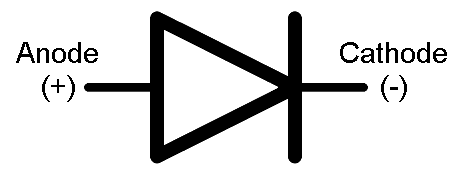
\includegraphics[width=0.25\linewidth]{./ImageFiles/Laboratorio 2/diodo_1}
	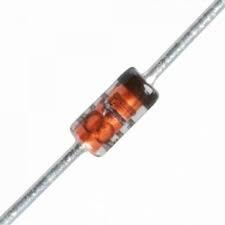
\includegraphics[width=0.15\linewidth]{./ImageFiles/Laboratorio 2/diodo_4}
	\caption{Rappresentazione simbolica di un diodo e foto del diodo 1N4148.}
	\label{fig:diodo}
\end{figure}
Il diodo è un dipolo che permette di realizzare circuiti raddrizzatori grazie al suo comportamento che differisce in base alle condizioni del circuito in cui è inserito. In particolare, se la tensione all'anodo è maggiore di una certa tensione di soglia (tipicamente considerata pari a \SI{0.7}{\volt}) rispetto alla tensione a cui si trova il catodo, il diodo permette il passaggio di corrente dall'anodo al catodo. Al contrario, non è consentito il passaggio di corrente dal catodo all'anodo. Più precisamente, la relazione corrente-tensione è descritta dalla seguente legge esponenziale:
\begin{equation}
	I_D=I_S[e^{\frac{V_D}{V_T}}-1],
\end{equation}
dove $I\sub{D}$ è la corrente nel diodo (con verso positivo dall'anodo al catodo), $I\sub{S}$ è la corrente inversa, $V\sub{D}$ è la differenza di tensione tra anodo e catodo mentre $V\sub{T}$ è la tensione termica. In figura \ref{fig:diodo_caratteristica} è rappresentata la caratteristica corrente-tensione dei due modelli del diodo: quello ideale e quello reale. In particolare, si definisce regione di funzionamento diretta quando il diodo è acceso e permette il passaggio di corrente da anodo a catodo ($V_{D}>0$) e regione inversa quando il diodo è spento e impedisce il passaggio di corrente (o più precisamente, la corrente è pari a $-I\sub{S}$).
\begin{figure}[tbh]
	\centering
	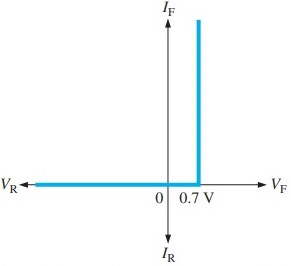
\includegraphics[width=0.3\linewidth]{./ImageFiles/Laboratorio 2/diodo_2}
	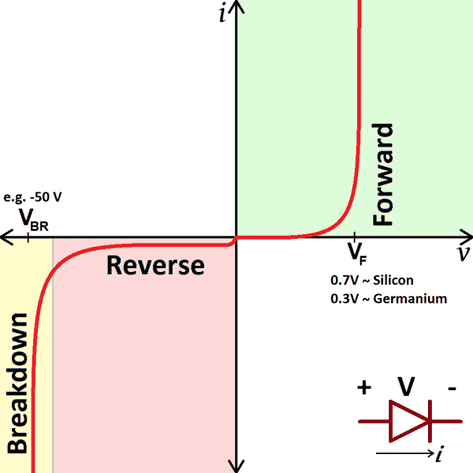
\includegraphics[width=0.3\linewidth]{./ImageFiles/Laboratorio 2/diodo_3}
	\caption{Caratteristica corrente-tensione del modello ideale (sinistra) e reale (destra) di un diodo.}
	\label{fig:diodo_caratteristica}
\end{figure}

Il primo circuito realizzato è un semplice raddrizzatore a singola semionda che utilizza un unico diodo e una resistenza. Lo schema del circuito è riportato in figura \ref{fig:circuito_1}.
\begin{figure}[h]
	\centering
	\begin{minipage}{.45\textwidth}
	\scalebox{1.4}{
		\begin{circuitikz}
			\draw (0,0) node[above]{$v_{in}$} to[short,o-] ++(1,0) to[D=$D$] ++(1,0) -- ++(.5,0) coordinate(dout) to[short, -o] ++(1,0) node[above]{$v_{out}$};
			\draw (dout) to[R=$R$] ++(0,-2) node[ground]{};
			\draw (-.5,-3) rectangle (4,1);
		\end{circuitikz}
	}
	\end{minipage}\qquad
	\begin{minipage}{.48\textwidth}
	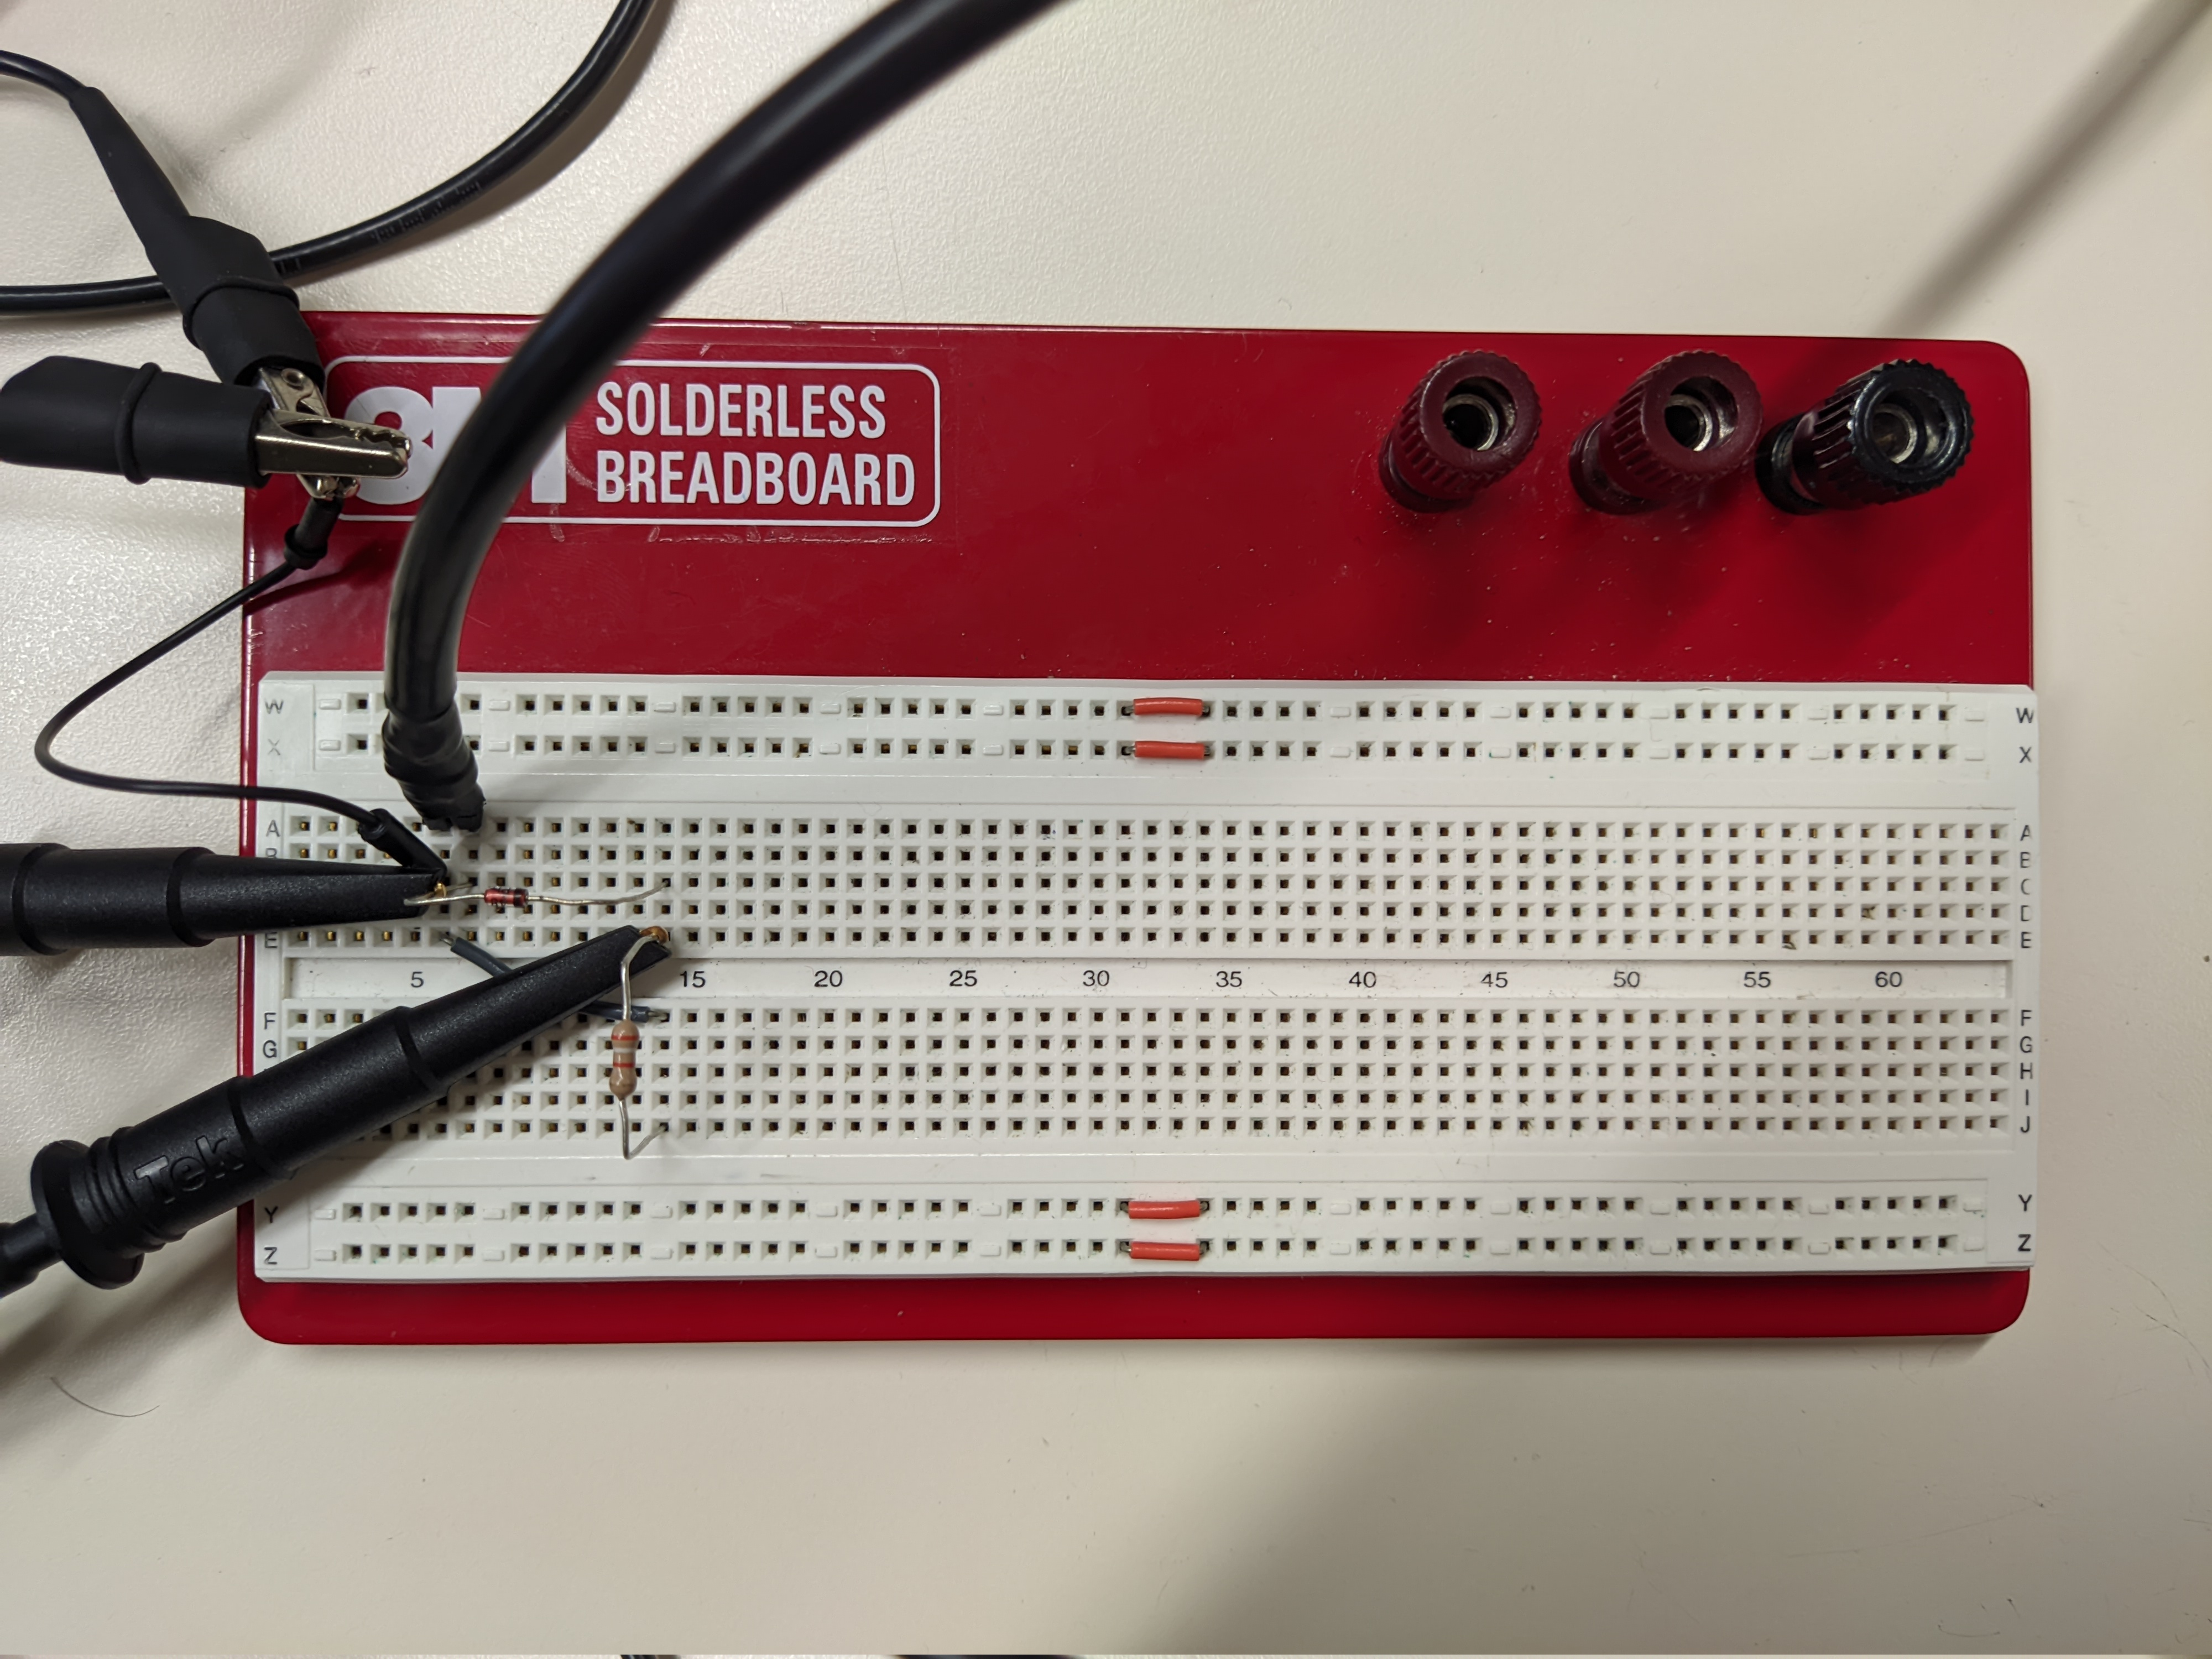
\includegraphics[width=\linewidth]{./ImageFiles/Laboratorio 2/CIR1.jpg}
	\end{minipage}
	\caption{Schema circuitale del raddrizzatore a singola semionda e foto del circuito realizzato.}
	\label{fig:circuito_1}
\end{figure}
Considerando il modello ideale del diodo, è possibile analizzare il comportamento del circuito quando in ingresso è applicata una tensione sinusoidale. Considerando una tensione di soglia del diodo pari a \SI{0.7}{\volt} si ha che:
\begin{itemize}
	\item se $v_{in}<\SI{0.7}{\volt}$ allora $v\sub{out}=\SI{0}{\volt}$, poiché nel circuito non scorre corrente, nemmeno nella resistenza R che quindi mantiene a massa il nodo $v\sub{out}$;
	\item se $v_{in} >= \SI{0.7}{\volt}$ il diodo $D$ si accende, quindi il nodo $v\sub{out}$ si porta a $v_{out}=v_{in}-\SI{0.7}{\volt}$.
\end{itemize}
Per analizzare il comportamento del circuito si sono effettuate delle misure tramite l'oscilloscopio sui nodi $v\sub{in}$ e $v\sub{out}$, applicando in ingresso sul nodo $v\sub{in}$ una sinusoide di ampiezza picco-picco pari a \SI{2}{\volt} e variando il valore della resistenza e della frequenza del segnale in ingresso. Nella tabella \ref{tab:valori_componenti_1} sono indicati i valori nominali e misurati delle resistenze utilizzate. \`E stata inoltre misurata la tensione di soglia del diodo utilizzato, che è risultata essere pari a \SI{0.618}{\volt}.

\def\arraystretch{1.3}
\begin{table}[h]
	\centering
	\begin{tabular}{|c|c|c|}
		\hline
		Componente	& Valore Nominale & Valore Misurato \\ \hline
		R\sub{1}          & \SI{12}{\kilo\ohm} &     \SI{11.95}{\kilo\ohm}  \\ \hline
		R\sub{2}          & \SI{39}{\kilo\ohm} &     \SI{38.11}{\kilo\ohm} \\ \hline
		R\sub{3}          & \SI{56}{\kilo\ohm} &     \SI{54.86}{\kilo\ohm} \\ \hline
		R\sub{4}          & \SI{110}{\kilo\ohm} &     \SI{109.73}{\kilo\ohm} \\ \hline
	\end{tabular}
	\caption{Valori nominali e misurati delle resistenze utilizzate nel circuito.}
	\label{tab:valori_componenti_1}
\end{table}

\noindent
Nella figura \ref{fig:voutvsresistance} sono rappresentate le differenti misure effettuate a frequenza fissa pari a \SI{1}{\kilo\hertz}, variando la resistenza utilizzata.
\begin{figure}[h]
	\centering
	\begin{minipage}{.496\textwidth}
				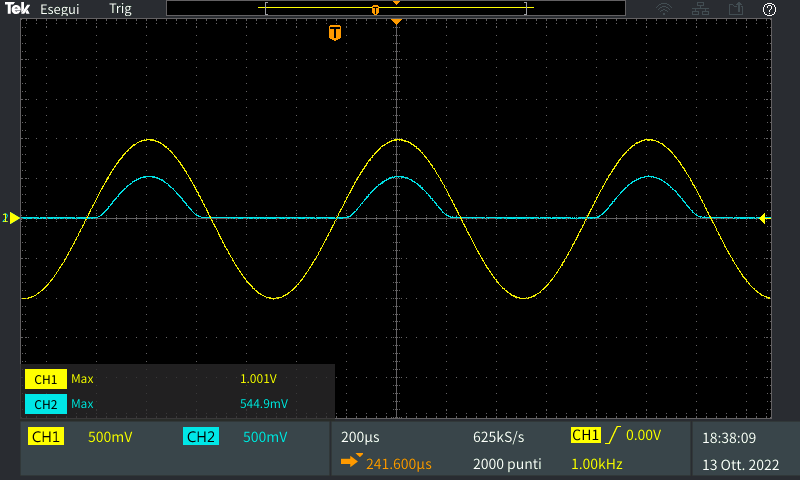
\includegraphics[width=\linewidth]{./ImageFiles/Laboratorio 2/TEK00000.PNG}
	\end{minipage}
	\begin{minipage}{.496\textwidth}
		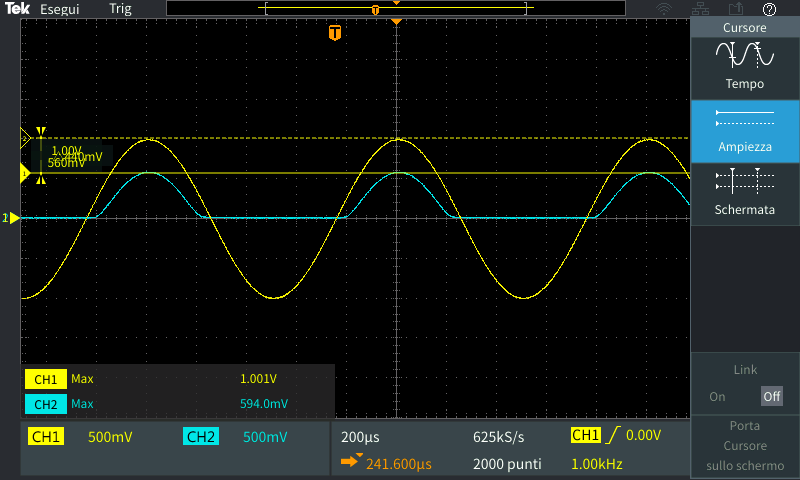
\includegraphics[width=\linewidth]{./ImageFiles/Laboratorio 2/TEK00009.PNG}
	\end{minipage}
	\begin{minipage}{.496\textwidth}
	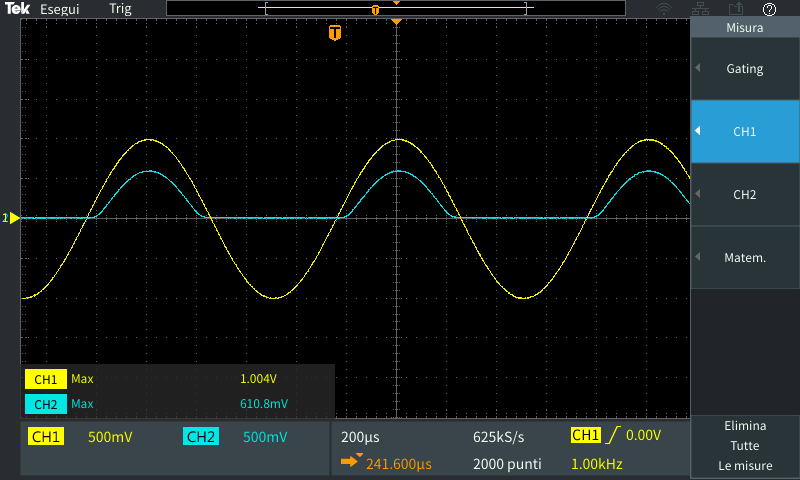
\includegraphics[width=\linewidth]{./ImageFiles/Laboratorio 2/TEK00003.PNG}
\end{minipage}
\begin{minipage}{.496\textwidth}
	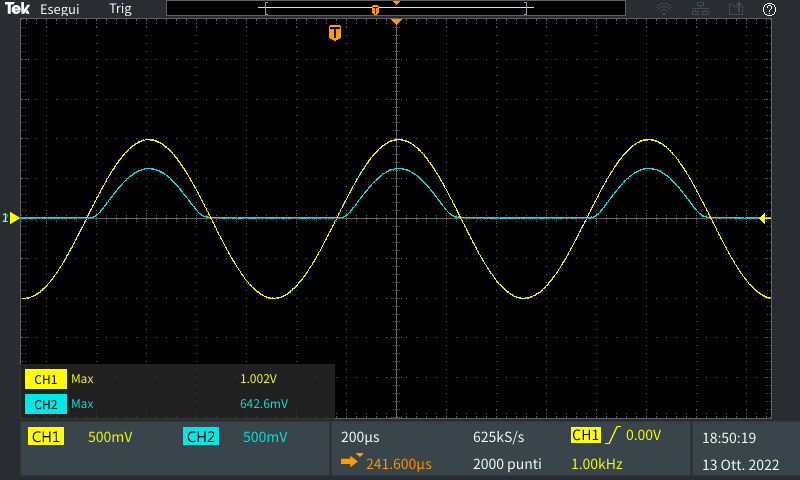
\includegraphics[width=\linewidth]{./ImageFiles/Laboratorio 2/TEK00007.PNG}
\end{minipage}
	\caption{Misure del segnale in ingresso (linea gialla) e del segnale in uscita (linea azzurra) al circuito. Il segnale in ingresso è una sinusoide di \SI{2}{\volt} picco-picco e frequenza pari a \SI{1}{\kilo\hertz}. La resistenza invece è pari a \SI{12}{\kilo\ohm} (in alto a sinistra), \SI{39}{\kilo\ohm} (in alto a destra), \SI{56}{\kilo\ohm} (in basso a sinistra) e \SI{110}{\kilo\ohm} (in basso a destra).}
	\label{fig:voutvsresistance}
\end{figure}
Come si può osservare, in un diodo reale c'è una dipendenza della tensione di soglia dalla corrente che lo attraversa: infatti, aumentando la resistenza diminuisce la corrente che circola nel circuito e quindi anche la tensione di soglia. Al contrario, diminuendo il valore della resistenza $R$ aumenta la corrente che circola nel circuito e quindi aumenta la tensione di soglia.
Successivamente si è analizzato il comportamento in frequenza del circuito, variando la frequenza della sinusoide in ingresso. Per le misure, si sono scelte le frequenze di \SI{1}{\kilo\hertz}, \SI{10}{\kilo\hertz}, \SI{100}{\kilo\hertz} e \SI{1}{\mega\hertz}, (\Fig\ref{fig:freqwith38}).
\begin{figure}[tbh]
	\centering
	\begin{minipage}{.496\textwidth}
		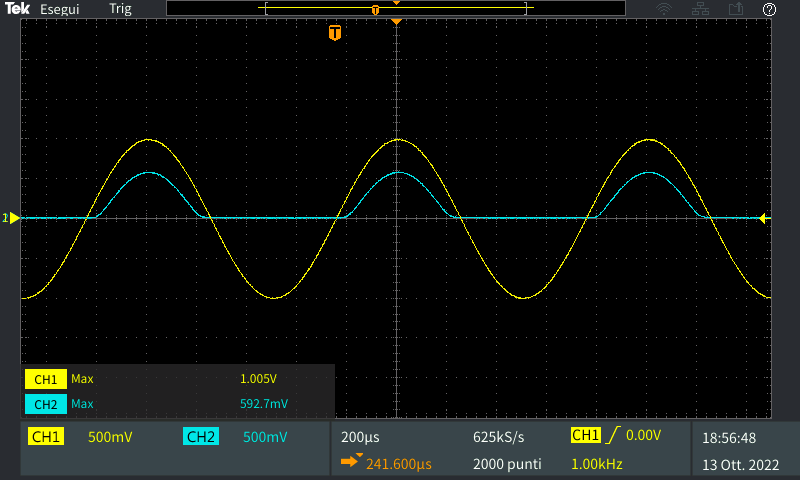
\includegraphics[width=\linewidth]{./ImageFiles/Laboratorio 2/TEK00011.PNG}
	\end{minipage}
	\begin{minipage}{.496\textwidth}
		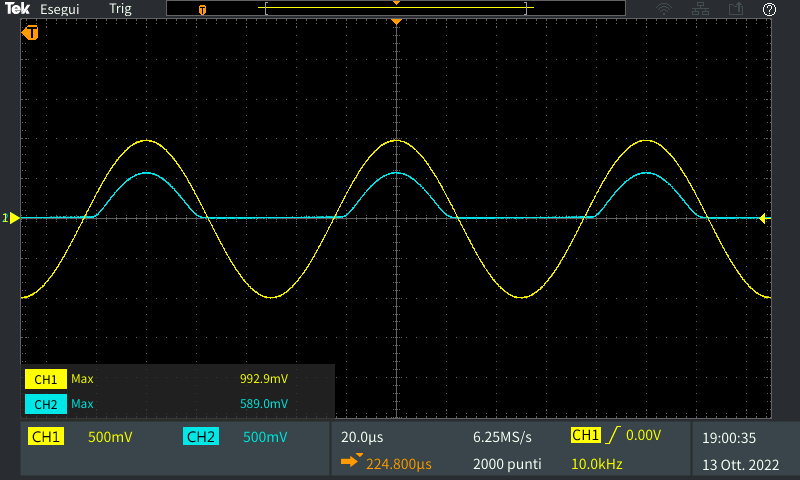
\includegraphics[width=\linewidth]{./ImageFiles/Laboratorio 2/TEK00012.PNG}
	\end{minipage}
	\begin{minipage}{.496\textwidth}
		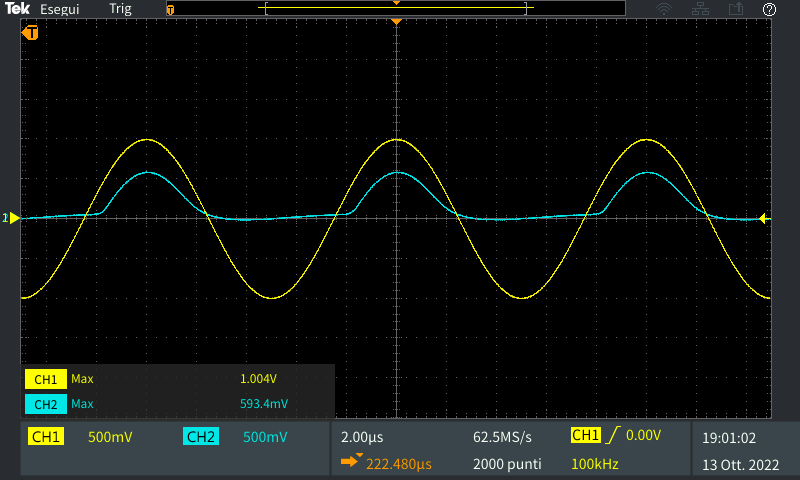
\includegraphics[width=\linewidth]{./ImageFiles/Laboratorio 2/TEK00013.PNG}
	\end{minipage}
	\begin{minipage}{.496\textwidth}
		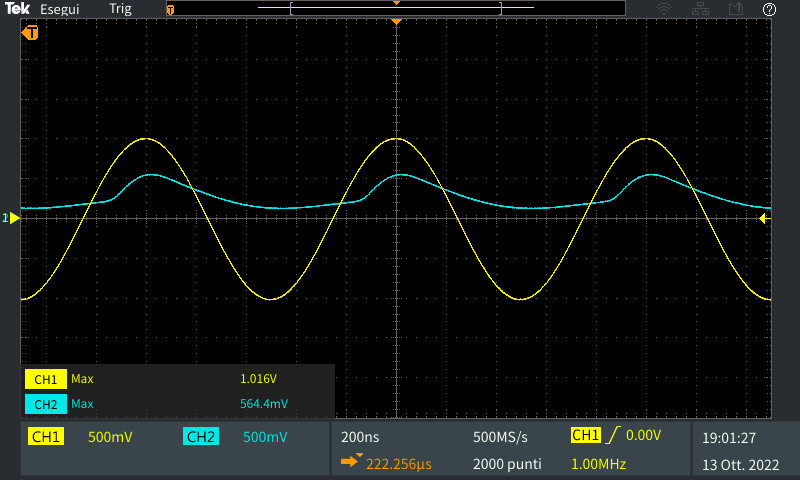
\includegraphics[width=\linewidth]{./ImageFiles/Laboratorio 2/TEK00014.PNG}
	\end{minipage}
	\caption{Misure del segnale in ingresso (linea gialla) e del segnale in uscita (linea azzurra) al circuito. La resistenza è fissa in tutti e quattro i grafici ed è pari a \SI{39}{\kilo\ohm} mentre la frequenza del segnale in ingresso è pari a \SI{1}{\kilo\hertz} (in alto a sinistra), \SI{10}{\kilo\hertz} (in alto a destra), \SI{100}{\kilo\hertz} (in basso a sinistra) e \SI{1}{\mega\hertz} (in basso a destra).}
	\label{fig:freqwith38}
\end{figure}
Osservando le acquisizioni si nota che aumentando la frequenza il segnale in uscita presenta una semionda distorta. In particolare, si può notare che il diodo riesce a seguire abbastanza correttamente il fronte di salita del segnale in ingresso (il diodo in questa fase si accende). Tuttavia, il diodo non è sufficientemente veloce nella fase di spegnimento: di conseguenza, il segnale in uscita dal diodo fa più fatica a seguire il segnale in ingresso\todo{non so come dirla meglio vediamo.}. Questo comportamento asimmetrico è presente a causa dei differenti tempi di accensione e spegnimento che caratterizzano un diodo reale. Questi intervalli sono determinati dai tempi necessari alla formazione ed eliminazione della regione di svuotamento nella giunzione P-N durante il passaggio dalla regione diretta a quella inversa del diodo.  

\clearpage

Un problema del circuito precedente è la presenza di un offset significativo tra la tensione $v\sub{in}$ e $v\sub{out}$: tale valore è pari alla tensione di soglia del diodo che varia a seconda delle condizioni del circuito in cui il diodo è inserito. Per eliminare questo problema si può utilizzare un circuito diverso che, utilizzando un amplificatore operazionale, consente di eliminare l'offset. Lo schema del circuito è presentato in figura \ref{fig:circuito_2}.
\begin{figure}[h]
	\centering
	\begin{minipage}{.45\textwidth}
		\scalebox{.8}{
			\begin{circuitikz}
				\draw (1,0) node[op amp, anchor=+](oa){\texttt{TL071}};
				\draw (0,0) node[above]{$v_{in}$} to[short,o-] (oa.+);
				\draw (oa.out) node[above]{$v_1$} to[short, o-] (oa.out) to[D=$D$] ++(3,0) coordinate (vout) to[short, -o] ++(1,0) node[above]{$v_{out}$};
				\draw (oa.-) node[left]{$v_-$} to[short, o-] ++(0,2) -| (vout);
				\draw (vout) to[R=$R$] ++(0,-2) node[ground]{};
				\draw [thick] (-.5,-3) rectangle (8,4);
			\end{circuitikz} 
		}
	\end{minipage}\qquad
	\begin{minipage}{.48\textwidth}
		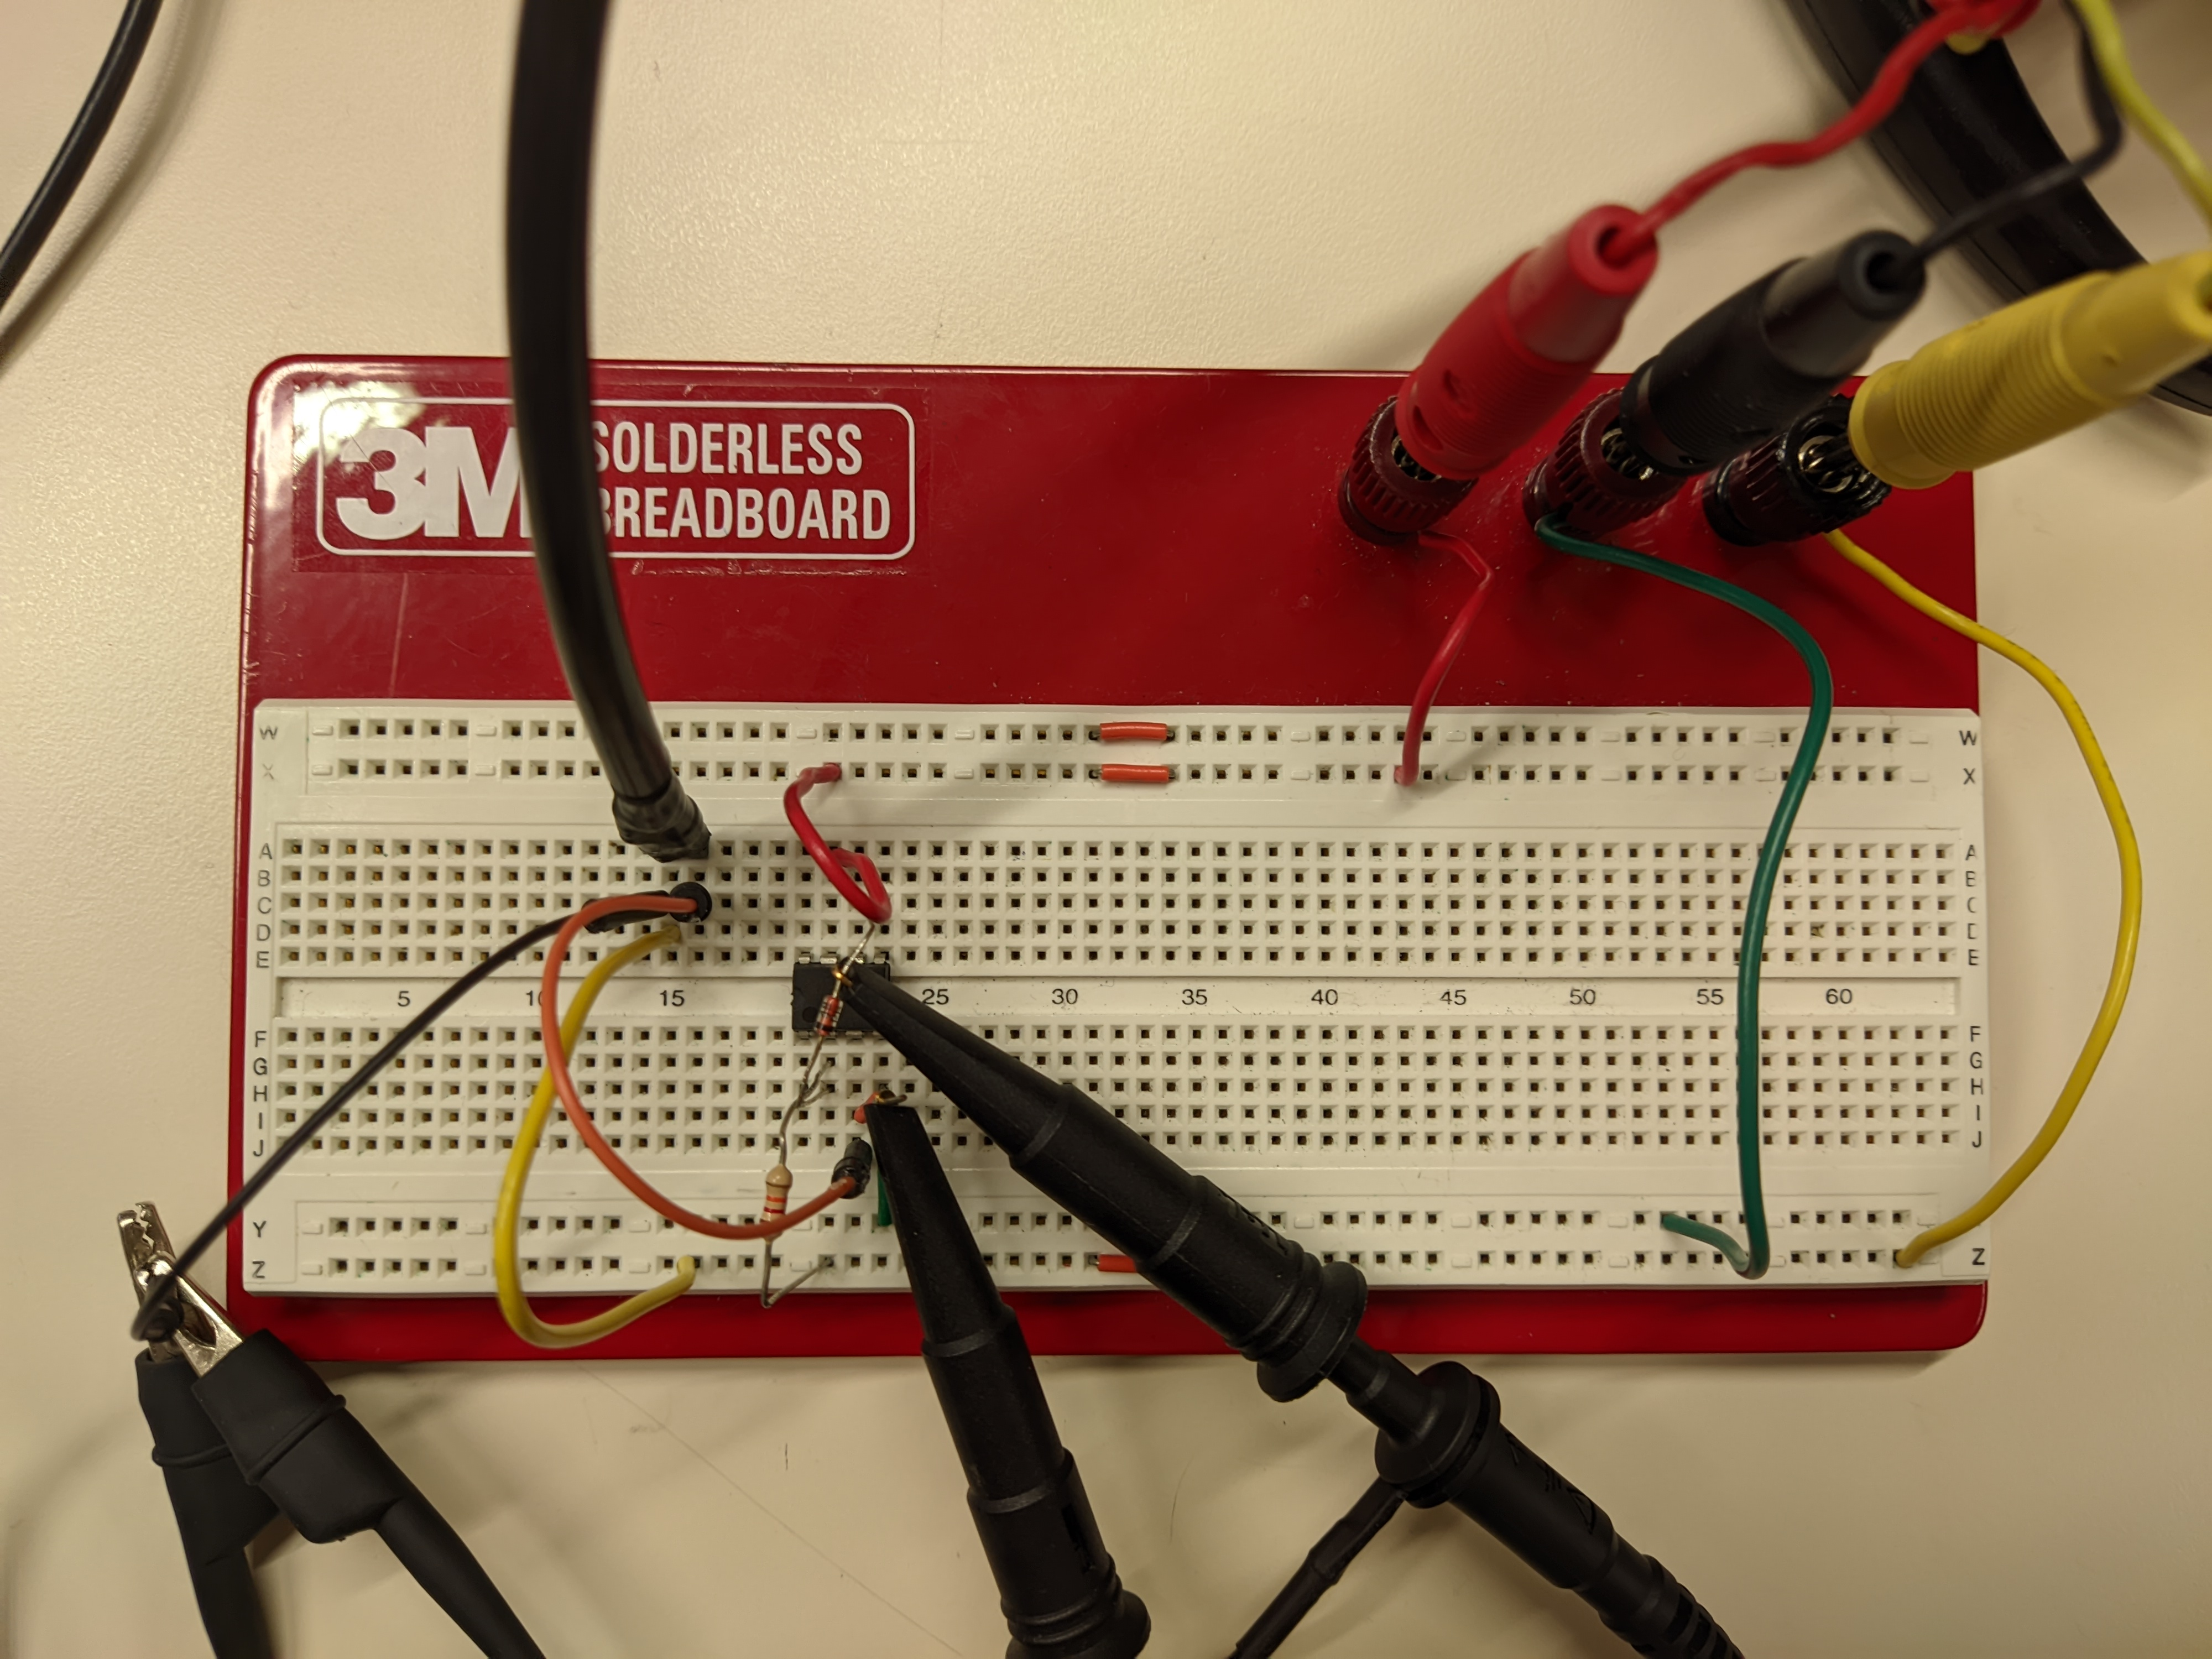
\includegraphics[width=\linewidth]{./ImageFiles/Laboratorio 2/CIR2.jpg}
	\end{minipage}
	\caption{Schema circuitale del raddrizzatore a singola semionda con amplificatore operazionale e foto del circuito realizzato.}
	\label{fig:circuito_2}
\end{figure}

Per analizzare il circuito, è utile considerarne il comportamento in due casi:
\begin{itemize}
	\item se $v_{in}>=0$, il diodo $D$ è acceso e il circuito si comporta come un buffer di tensione. Essendo $v_{out}=v_{in}>0$, avremo una corrente nella resistenza $R$ che scorre verso massa. Questa corrente è fornita dall'amplificatore operazionale e quindi polarizza il diodo. La tensione $v\sub{1}$ sarà invece pari a $v_1=v_{out}+V_D=v_{out}+\SI{0.7}{\volt}$;
	\item se $v_{in}<0$, il diodo $D$ è spento e l'amplificatore operazionale non è più retroazionato. All'interno della resistenza non scorre corrente e quindi il nodo $v\sub{out}$ è mantenuto a una tensione di \SI{0}{\volt}. In questo caso, l'amplificatore operazionale si comporta come un comparatore: essendo $v\sub{in}$ negativa, $v\sub{1}$ si porta alla tensione di saturazione negativa dell'amplificatore.
\end{itemize}

\noindent
In figura \ref{fig:analisi_circuito_2_1} è possibile osservare le misure di v\sub{in} e v\sub{1} eseguite per mezzo dell'oscilloscopio. Si noti inoltre che, tramite la funzione \textit{Min} dell'oscilloscopio, è stata misurata la tensione di saturazione negativa dell'amplificatore operazionale. Essa è pari a -\SI{8.589}{\volt}.
\begin{figure}[h]
	\centering
	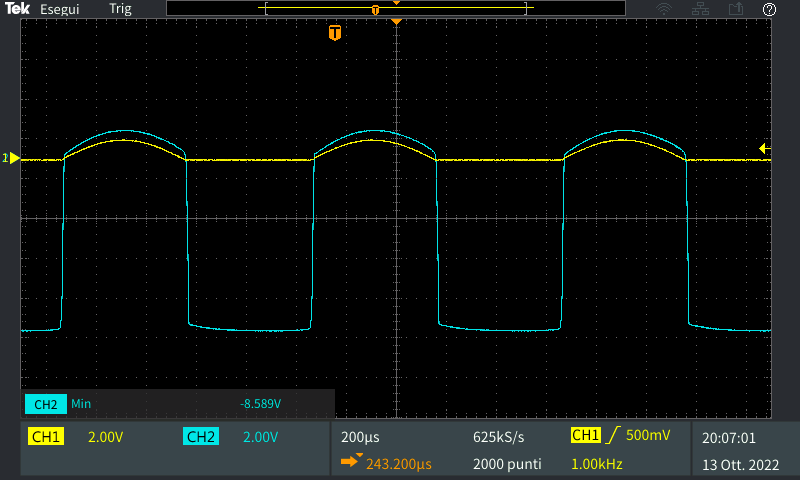
\includegraphics[width=1\linewidth]{./ImageFiles/Laboratorio 2/TEK00030}
	\caption{Misure del segnale $v_{in}$ (linea gialla) e del segnale $v_{1}$ (linea azzurra). Si è utilizzata in ingresso un segnale sinusoidale di ampiezza picco-picco \SI{2}{\volt} con frequenza pari a \SI{1}{\kilo\hertz}.}
	\label{fig:analisi_circuito_2_1}
\end{figure}

\noindent
In questo circuito, si è mantenuto costante il valore di $R$, mentre si è variata la frequenza del segnale in ingresso \ref{fig:freqseccirc}.
\begin{figure}[h]
	\centering
	\begin{minipage}{.496\textwidth}
		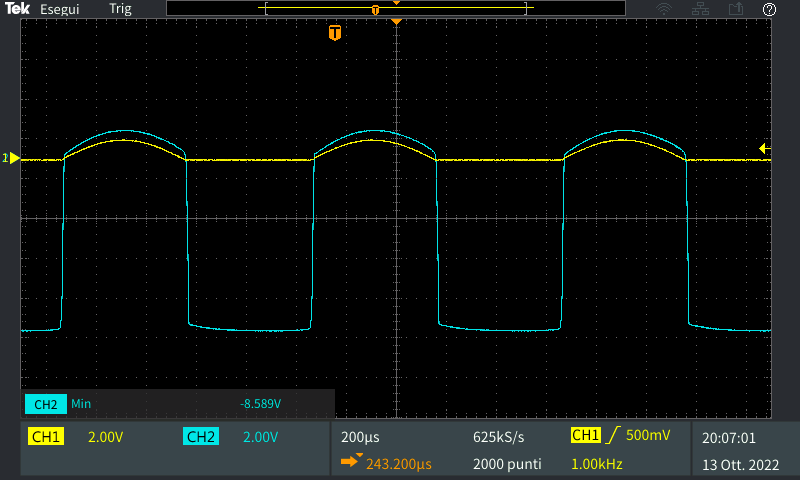
\includegraphics[width=\linewidth]{./ImageFiles/Laboratorio 2/TEK00030.PNG}
	\end{minipage}
	\begin{minipage}{.496\textwidth}
		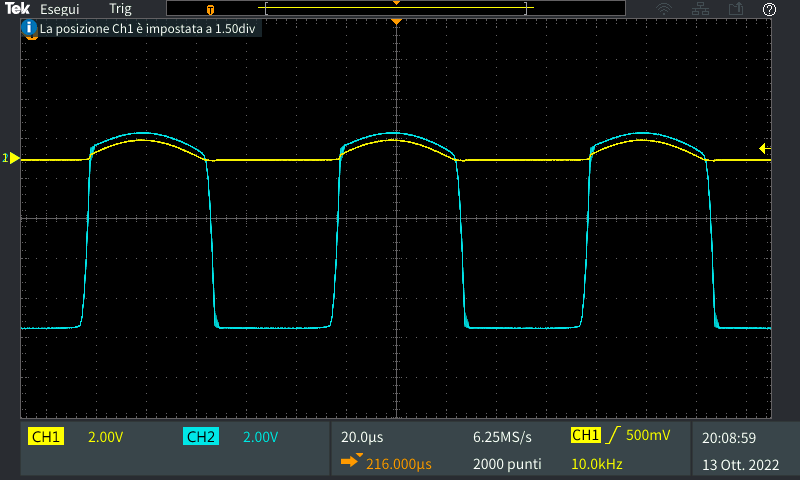
\includegraphics[width=\linewidth]{./ImageFiles/Laboratorio 2/TEK00032.PNG}
	\end{minipage}
	\begin{minipage}{.496\textwidth}
		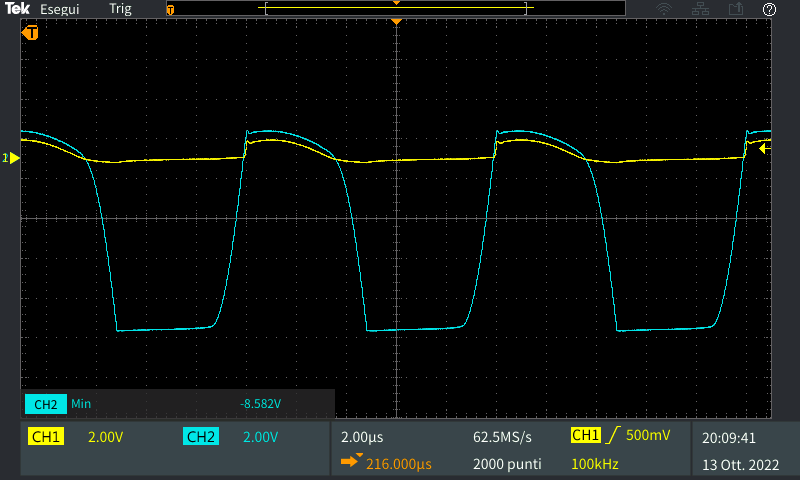
\includegraphics[width=\linewidth]{./ImageFiles/Laboratorio 2/TEK00034.PNG}
	\end{minipage}
	\begin{minipage}{.496\textwidth}
		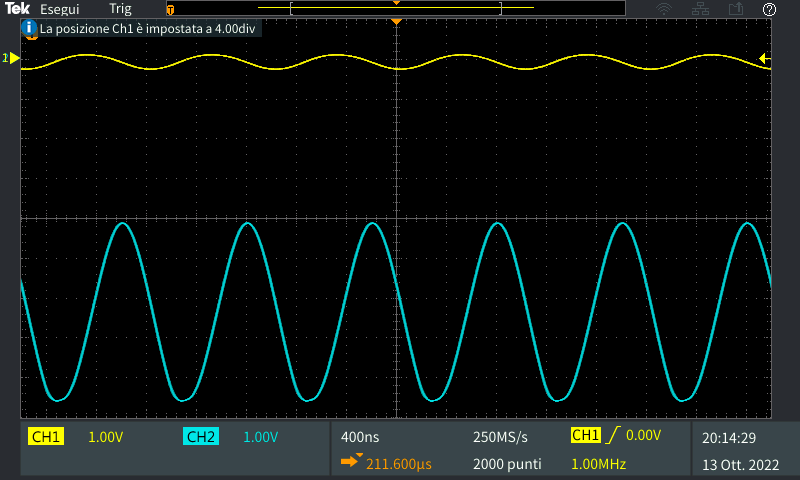
\includegraphics[width=\linewidth]{./ImageFiles/Laboratorio 2/TEK00036.PNG}
	\end{minipage}
	\caption{Misure del segnale $v_{out}$ (linea gialla) e del segnale $v_{1}$ (linea azzurra). Si è utilizzato in ingresso un segnale sinusoidale con ampiezza picco-picco di \SI{2}{\volt} e frequenza di \SI{1}{\kilo\hertz} (in alto a sinistra), \SI{10}{\kilo\hertz} (in alto a destra), \SI{100}{\kilo\hertz} (in basso a sinistra) e \SI{1}{\mega\hertz} (in basso a destra).}
	\label{fig:freqseccirc}
\end{figure}

\noindent
Analizzando più in dettaglio il comportamento del circuito, si nota un ritardo di circa \SI{4.08}{\micro\second} sul fronte di salita dell'uscita rispetto all'ingresso (\Fig\ref{fig:slewrate}).
\begin{figure}[!h]
	\centering
	\begin{minipage}{.496\textwidth}
		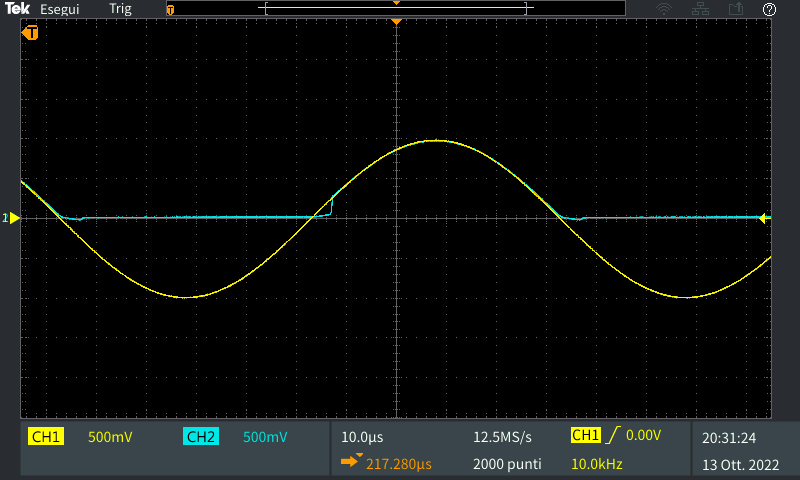
\includegraphics[width=\linewidth]{./ImageFiles/Laboratorio 2/TEK00038.PNG}
	\end{minipage}
	\begin{minipage}{.496\textwidth}
		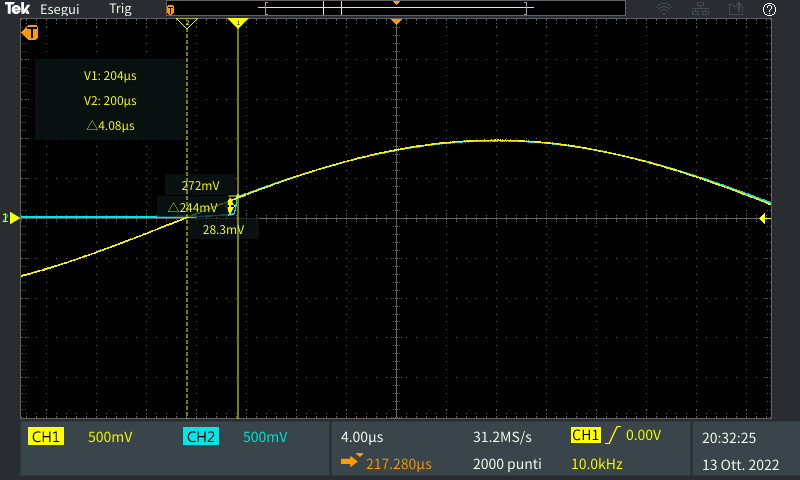
\includegraphics[width=\linewidth]{./ImageFiles/Laboratorio 2/TEK00039.PNG}
	\end{minipage}
	\caption{Misure del segnale $v_{in}$ (linea gialla) e del segnale $v_{out}$ (linea azzurra). Si può osservare il fenomeno dello \textit{slew rate} con un ritardo tra segnale in ingresso e uscita di circa \SI{4.08}{\micro\second} (figura a destra).}
	\label{fig:slewrate}
\end{figure}
Questo andamento è causato dal fatto che, non appena $v\sub{in}$ diventa maggiore di zero, l'uscita deve saltare dalla tensione di saturazione negativa al valore del segnale in ingresso. Il tempo necessario all'amplificatore per effettuare questa transizione è regolato da un parametro tipico degli amplificatori operazionali definito \textit{slew rate}: tale parametro indica la velocità massima con cui l'amplificatore operazionale può far variare la tensione alla sua uscita. Per questo motivo, lo \textit{slew rate} è misurato in $\frac{V}{\mu s}$ ed è specificato dal produttore all'interno del datasheet. Nel caso dell'amplificatore \textbf{TL071}, questo parametro può assumere valori da \SI{8}{\micro\second} a \SI{16}{\micro\second}. Si è cercato di stimare lo \textit{slew rate} nel circuito realizzato facendo il rapporto della differenza tra il valore finale raggiunto e la tensione di saturazione negativa con il tempo necessario ad effettuare questa transizione (\Fig\ref{fig:slewratevolt}):

\begin{equation}
	SR=\frac{\delta V}{\delta t}=\frac{\SI{9.64}{\volt}}{\SI{1.72}{\micro\second}}=5. 6\frac{V}{\mu s}.
\end{equation}
Il valore, pur non rientrando nell'intervallo specificato nel datasheet, assume un valore prossimo.
\begin{figure}[tbh]
	\centering
	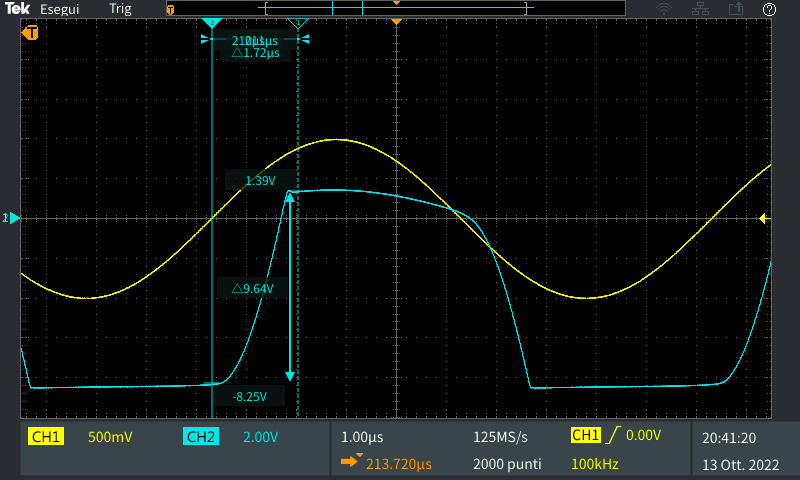
\includegraphics[width=\linewidth]{./ImageFiles/Laboratorio 2/TEK00040.PNG}
	\caption{Misure del segnale $v_{in}$ (linea gialla) e del segnale $v_{out}$ (linea azzurra). Si è utilizzata in ingresso un segnale sinusoidale di ampiezza picco-picco \SI{2}{\volt} con frequenza pari a \SI{10}{\kilo\hertz}. Sono stati utilizzati i cursori forniti dall'oscilloscopio per ottenere le variabili necessarie al calcolo dello \textit{slew rate}.}
	\label{fig:slewratevolt}
\end{figure}

\clearpage
Il circuito appena presentato elimina il problema dell'offset tra l'ingresso e l'uscita, ma introduce il ritardo causato dallo \textit{slew rate}. Inoltre, la semionda negativa viene completamente persa. Di seguito, si riporta lo schema del terzo circuito realizzato in laboratorio (\Fig\ref{fig:circuito_3}). Esso svolge la funzione di raddrizzatore a doppia semionda, risolvendo il problema causato dallo \textit{slew rate}, introducendo però l'offset tra ingresso e uscita.

\begin{figure}[ht!]
	\centering
	\begin{minipage}{.45\textwidth}
		\scalebox{.658}{
			\begin{circuitikz}
    			\draw (0,-.5) node[ground]{};
				\draw (0,2) coordinate (vin) to[sV=$v_{in}$] (0,-.5);
				\draw (0,2) to[R=$R_1$] ++(3,0);
				\draw (3,2) to (4,2);
				\draw (3.7,2) node[op amp, anchor=-](oa){\texttt{TL071}};
				\draw (oa.up) -- ++(0, .3) node[vcc]{$+E$};
				\draw (oa.down) -- ++(0,-.3) node[vee]{$-E$};
				\draw (3,2) -- ++(0,2) coordinate(C) to[R=$R_2$] ++(3.08,0) (C-|oa.out) coordinate(Co) to[short, -o] (oa.out) coordinate(vmin) to[D=$D_1$] ++(2,0) coordinate(dout) to [short, -o] ++(1,0) ++(.1,.1) node[above]{$v_{out}$};
				\draw (vmin) ++(.1,-.1) node[below]{$v_1$};
				\draw (dout) to[R=$R_3$] ++(0,-2) coordinate(bottom) node[ground]{};
				\draw (3.7,-.5) node[ground]{} to[short, -*] (3.7,1);
				\draw (vin) -- ++(0,3.5) -- ++(1,0) to[D=$D_2$] ++(7,0) -| (dout);
				\draw[thick] (-1,-1.5) rectangle (9.65,6.5);
			\end{circuitikz} 
		}
	\end{minipage}\qquad
	\begin{minipage}{.45\textwidth}
		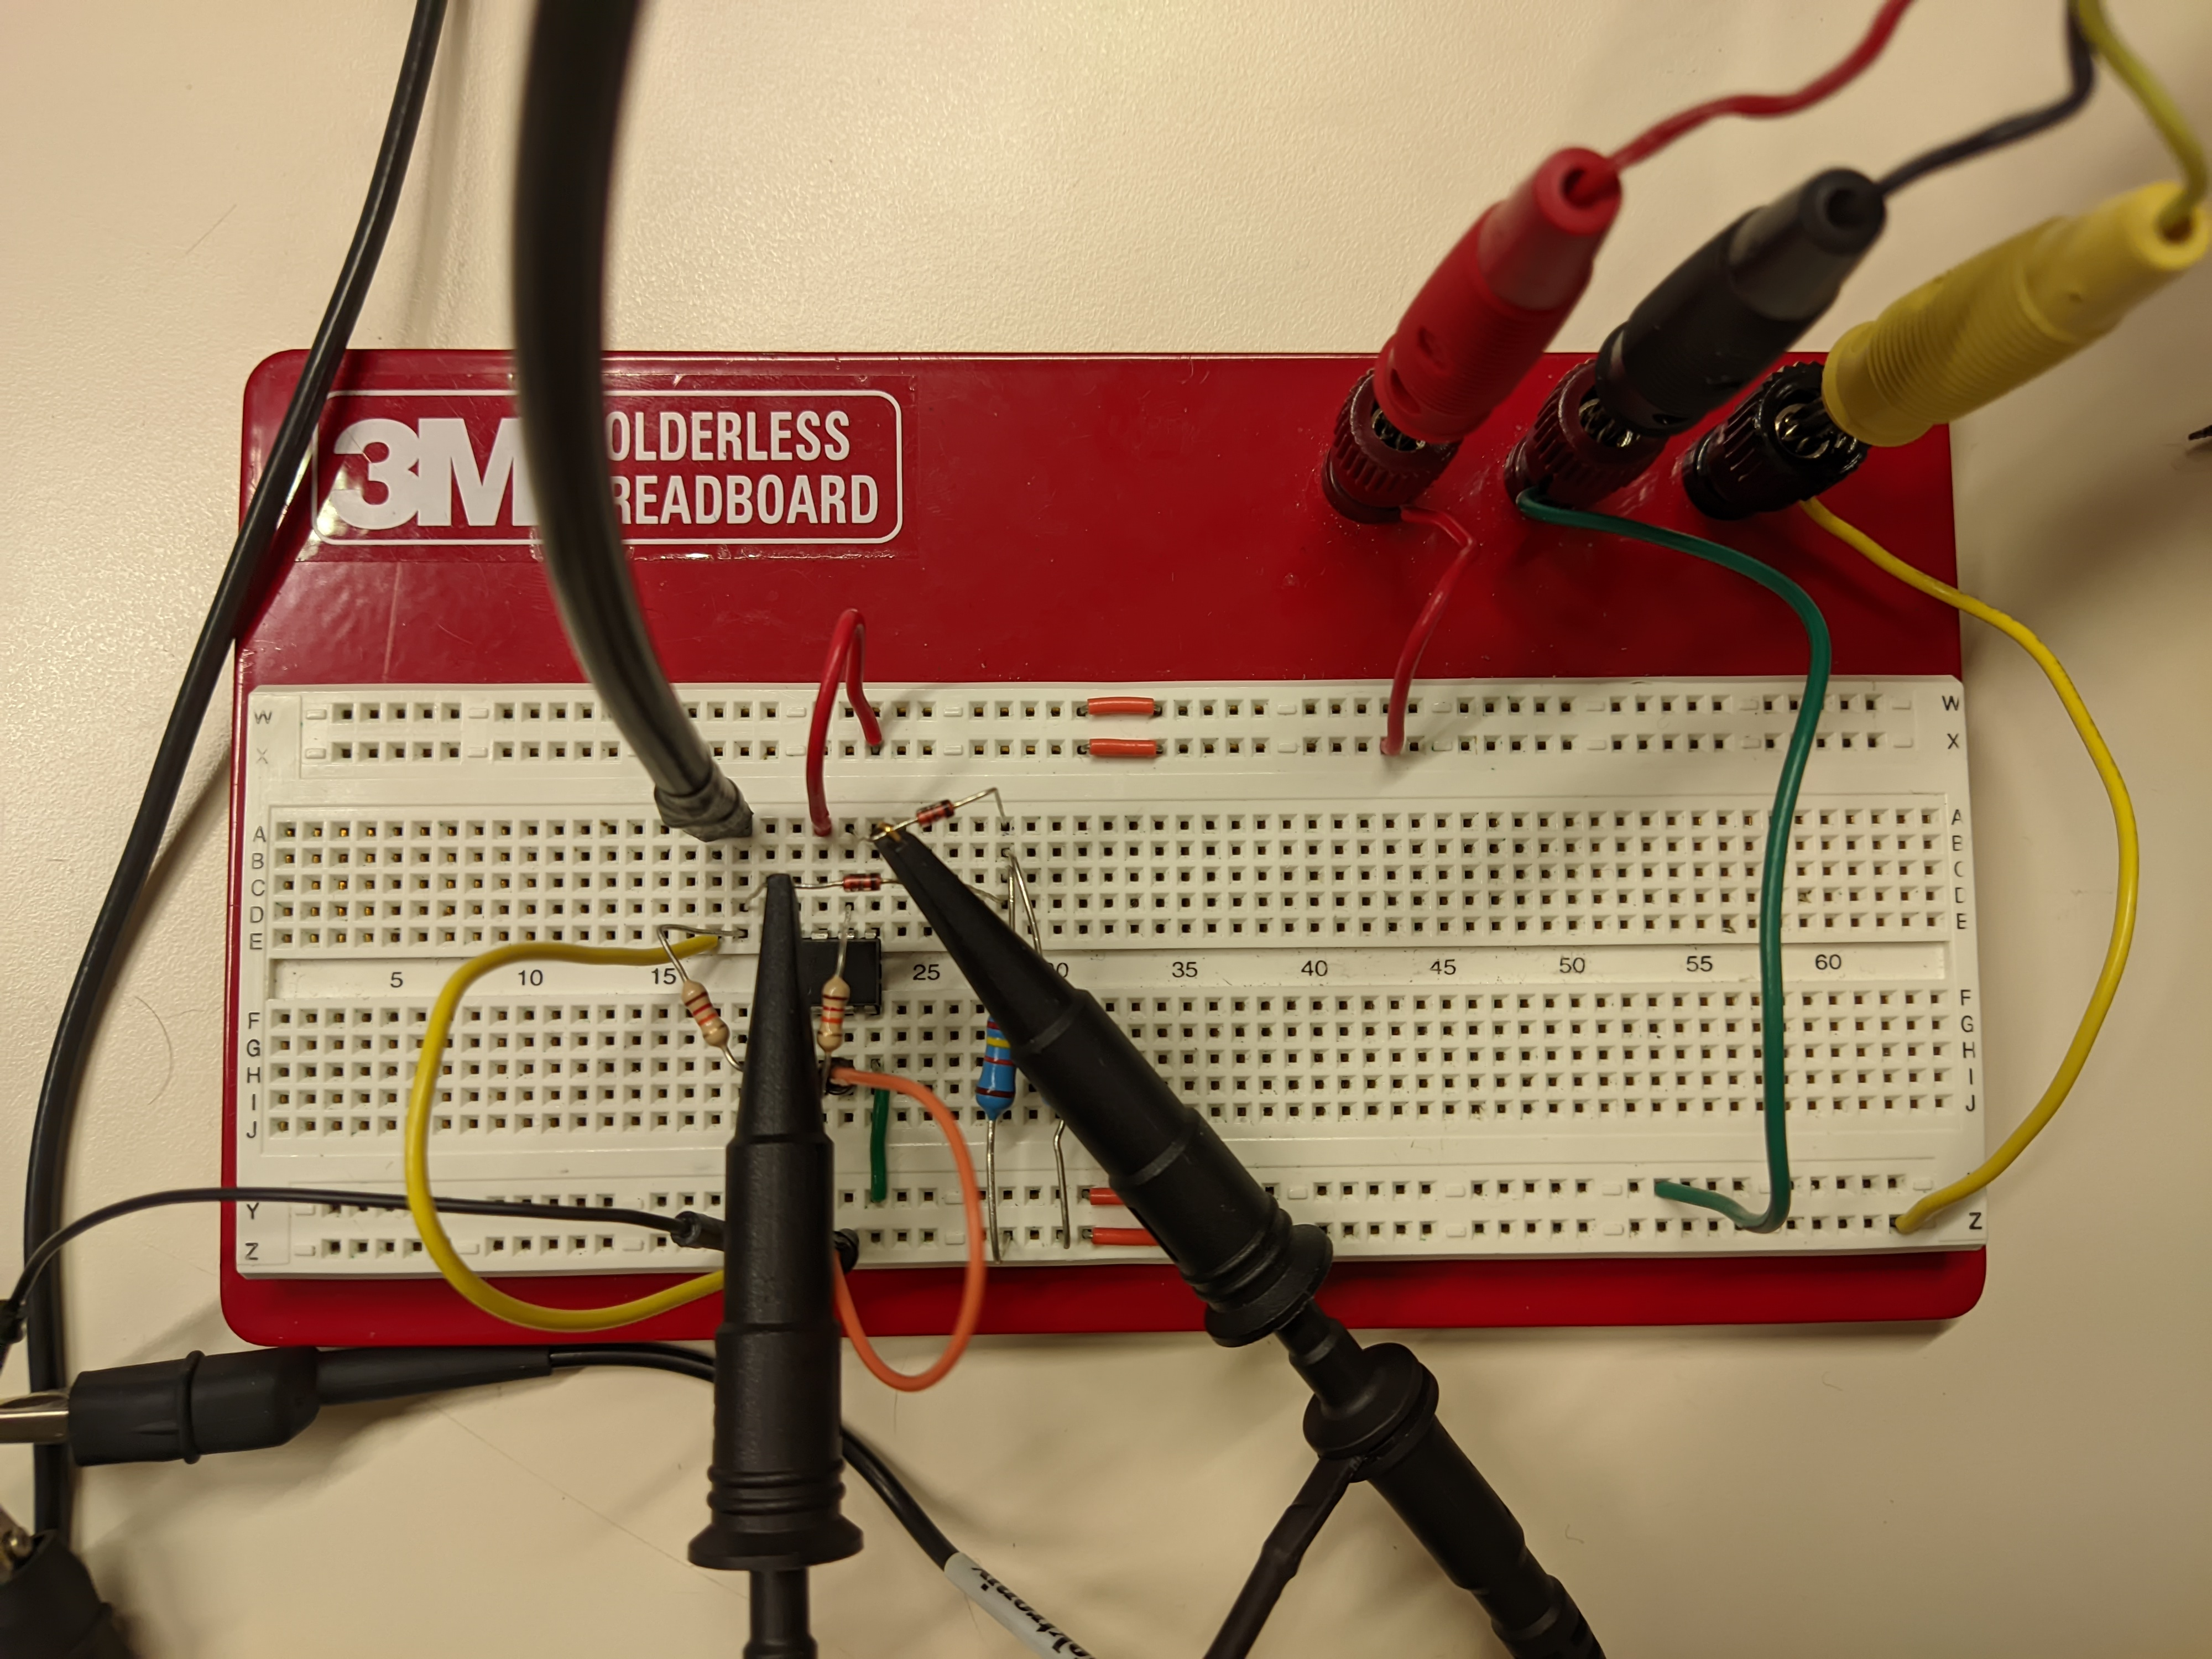
\includegraphics[width=\linewidth]{./ImageFiles/Laboratorio 2/CIR3.jpg}
	\end{minipage}
	\caption{Schema circuitale del raddrizzatore a doppia semionda e foto del circuito realizzato.}
	\label{fig:circuito_3}
\end{figure}

Si sono utilizzati due diodi 1N4148 con tensioni di soglia misurate pari a \todo{aggiungere tensioni di soglia} mentre si riportano nella tabella \ref{tab:valori_componenti_3} i valori nominali e misurati delle resistenze utilizzate.

\def\arraystretch{1.3}
\begin{table}[h!]
	\centering
	\begin{tabular}{|c|c|c|}
		\hline
		Componente	& Valore Nominale & Valore Misurato \\ \hline
		R\sub{1}          & \SI{12}{\kilo\ohm} &     \SI{11.95}{\kilo\ohm}  \\ \hline
		R\sub{2}          & \SI{12}{\kilo\ohm} &     \SI{38.11}{\kilo\ohm} \\ \hline
		R\sub{3}          & \SI{12}{\kilo\ohm} &     \SI{54.86}{\kilo\ohm} \\ \hline
	\end{tabular}
	\caption{Valori nominali e misurati delle resistenze utilizzate nel circuito.}
	\label{tab:valori_componenti_3}
\end{table}\todo{da inserire valori corretti}

Si può analizzare il circuito in due condizioni:
\begin{itemize}
	\item $v_{in}>=\SI{0.7}{\volt}$: in questo caso il diodo D\sub{2} è acceso mentre il diodo D\sub{1} è spento. Infatti, si può riconoscere che l'amplificatore operazionale è in configurazione di amplificatore invertente con guadagno unitario (pari a $\frac{R_2}{R_1}\simeq 1$). Per cui, avremo che $v_1=-v_{in}$. Per questo D\sub{1} è spento, mentre scorrerà corrente in D\sub{2} verso massa attraverso la resistenza R\sub{3};
	\item  $v_{in}<=-\SI{0.7}{\volt}$: D\sub{2} sarà spento in quanto la tensione tra anodo e catodo è inferiore alla tensione di soglia, mentre D\sub{1} sarà acceso, in quanto $v_1=-v_{in}>\SI{0.7}{\volt}$. Per cui, $v_{out}=v_1-\SI{0.7}{\volt}=-v_{in}-\SI{0.7}{\volt}$;
	\item $-\SI{0.7}{\volt}<v_{in}<\SI{0.7}{\volt}$: entrambi i diodi sono spenti e quindi $v_{out}=\SI{0}{\volt}$.
\end{itemize}

\noindent
Nelle figure \ref{fig:analisi_circuito_3_1} e \ref{fig:analisi_circuito_3_2} sono messi in evidenza il comportamento della tensione al nodo v\sub{out} e al nodo v\sub{1}.
\begin{figure}[h]
	\centering
	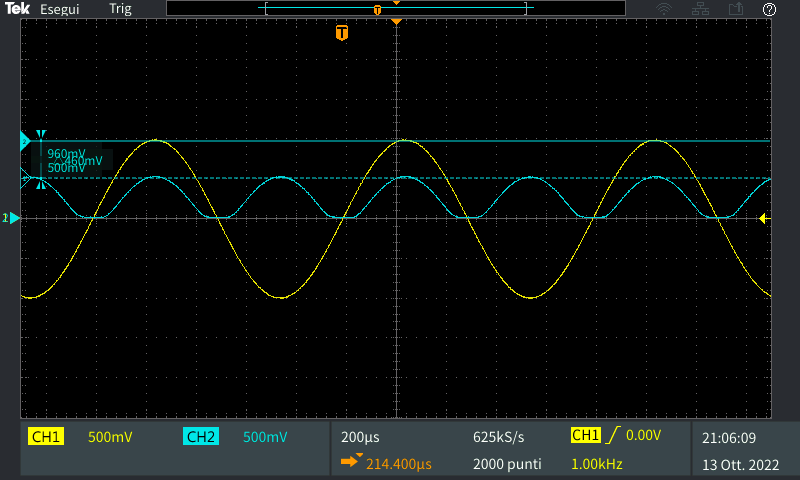
\includegraphics[width=1\linewidth]{./ImageFiles/Laboratorio 2/TEK00043}
	\caption{Misure del segnale $v_{in}$ (linea gialla) e del segnale $v_{out}$ (linea azzurra). Si è utilizzata in ingresso un segnale sinusoidale di ampiezza picco-picco \SI{2}{\volt} con frequenza pari a \SI{1}{\kilo\hertz}.}
	\label{fig:analisi_circuito_3_1}
\end{figure}
\begin{figure}[h]
	\centering
	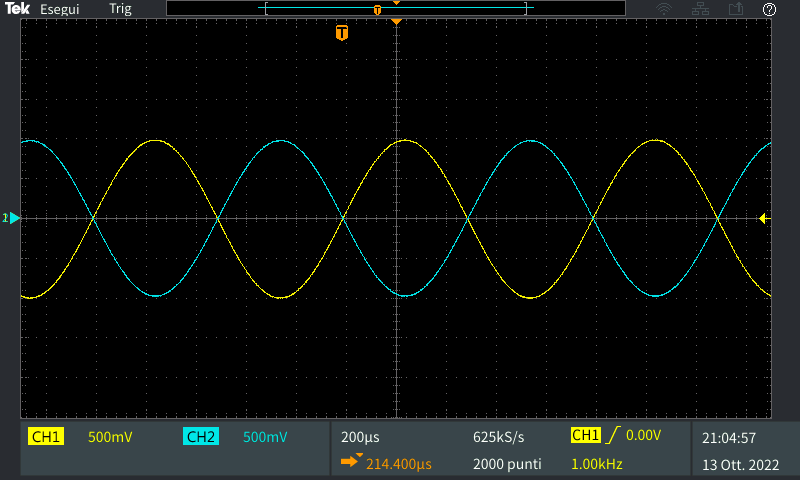
\includegraphics[width=1\linewidth]{./ImageFiles/Laboratorio 2/TEK00042}
	\caption{Misure del segnale $v_{in}$ (linea gialla) e del segnale $v_{1}$ (linea azzurra). Si è utilizzata in ingresso un segnale sinusoidale di ampiezza picco-picco \SI{2}{\volt} con frequenza pari a \SI{1}{\kilo\hertz}.}
	\label{fig:analisi_circuito_3_2}
\end{figure}

\noindent
Questa configurazione permette di rendere indipendente le prestazioni in frequenza del raddrizzatore dallo \textit{slew rate} del particolare amplificatore operazionale utilizzato. Infatti, la dipendenza del circuito del precedente circuito dal questo parametro era causata dal fatto che veniva interrotta la retroazione per $v_{in}<\SI{0}{\volt}$, portando l'uscita alla saturazione negativa. In questo circuito, l'amplificatore è sempre retroazionato e quindi la sua uscita non satura. Per questo motivo, il comportamento in frequenza del circuito dipende solamente dai tempi di accensione e spegnimento dei diodi utilizzati. 

\noindent
Per analizzare il comportamento in frequenza del circuito sono state fatte delle misure variando la frequenza del segnale sinusoidale da \SI{1}{\kilo\hertz} a \SI{1}{\mega\hertz} (\Fig\ref{fig:analisi_circuito_3_freq}).
\begin{figure}[!h]
	\centering
	\begin{minipage}{.496\textwidth}
		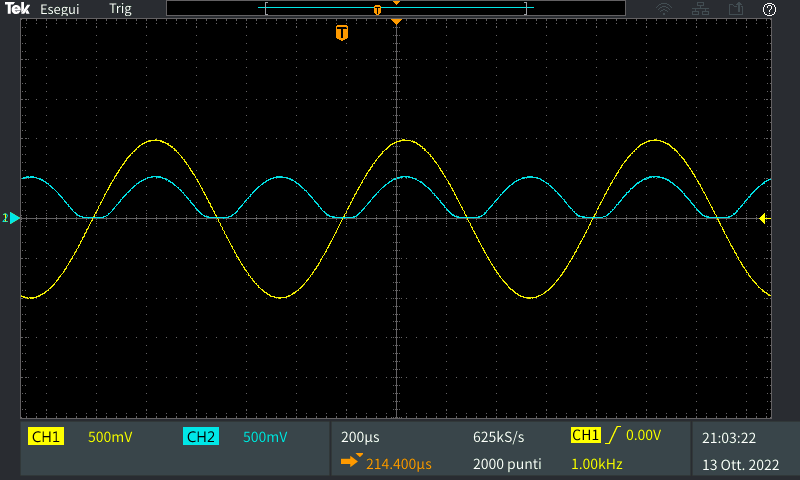
\includegraphics[width=\linewidth]{./ImageFiles/Laboratorio 2/TEK00041.PNG}
	\end{minipage}
	\begin{minipage}{.496\textwidth}
		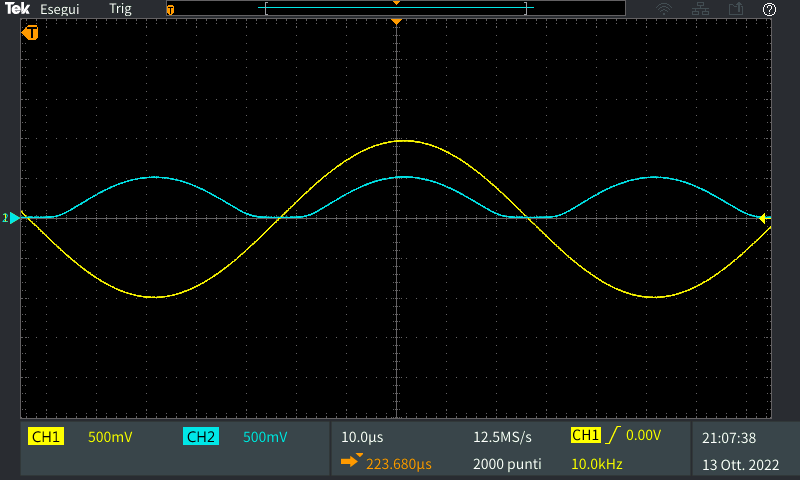
\includegraphics[width=\linewidth]{./ImageFiles/Laboratorio 2/TEK00046.PNG}
	\end{minipage}
	\begin{minipage}{.496\textwidth}
		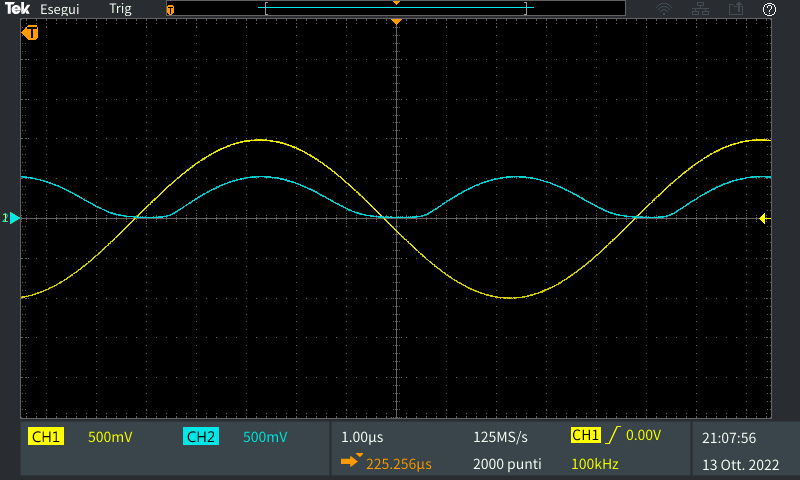
\includegraphics[width=\linewidth]{./ImageFiles/Laboratorio 2/TEK00047.PNG}
	\end{minipage}
	\begin{minipage}{.496\textwidth}
		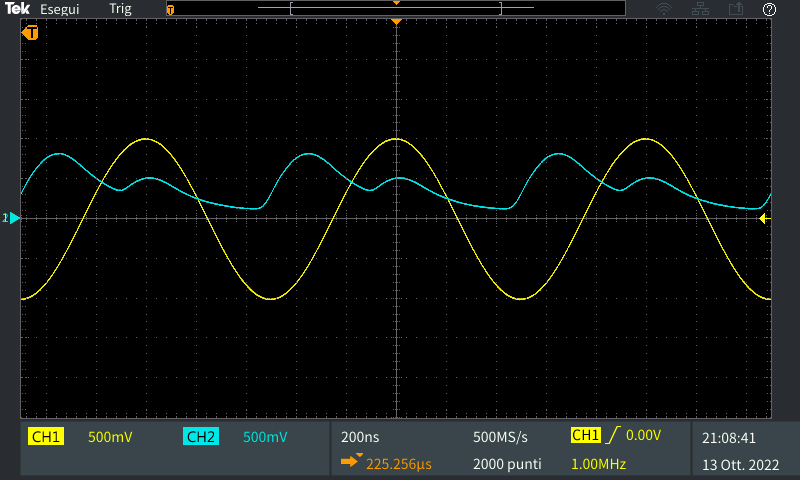
\includegraphics[width=\linewidth]{./ImageFiles/Laboratorio 2/TEK00048.PNG}
	\end{minipage}
	\caption{Misure del segnale $v_{in}$ (linea gialla) e del segnale $v_{out}$ (linea azzurra). Si è utilizzato in ingresso un segnale sinusoidale con ampiezza picco-picco di \SI{2}{\volt} e frequenza di \SI{1}{\kilo\hertz} (in alto a sinistra), \SI{10}{\kilo\hertz} (in alto a destra), \SI{100}{\kilo\hertz} (in basso a sinistra) e \SI{1}{\mega\hertz} (in basso a destra).}
	\label{fig:analisi_circuito_3_freq}
\end{figure}
Dai risultati ottenuti si può osservare come fino alla frequenza di \SI{100}{\kilo\hertz} il circuito funziona ancora correttamente, presentando in uscita una leggera distorsione del segnale. Alla frequenza di \SI{1}{\mega\hertz}, il segnale il uscita presenta una forte distorsione e il circuito non funziona più come un raddrizzatore. Infatti, analizzando più precisamente l'andamento di v\sub{1} e v\sub{in} (\Fig\ref{fig:analisi_circuito_3_3}), notiamo come il segnale v\sub{1} presenta uno sfasamento e, al contrario delle aspettative, presenta anche un fattore di amplificazione. Questo comportamento è complesso da descrivere in quanto bisognerebbe considerare il comportamento in frequenza dell'amplificatore operazionale e dei componenti passivi.
\begin{figure}[h]
	\centering
	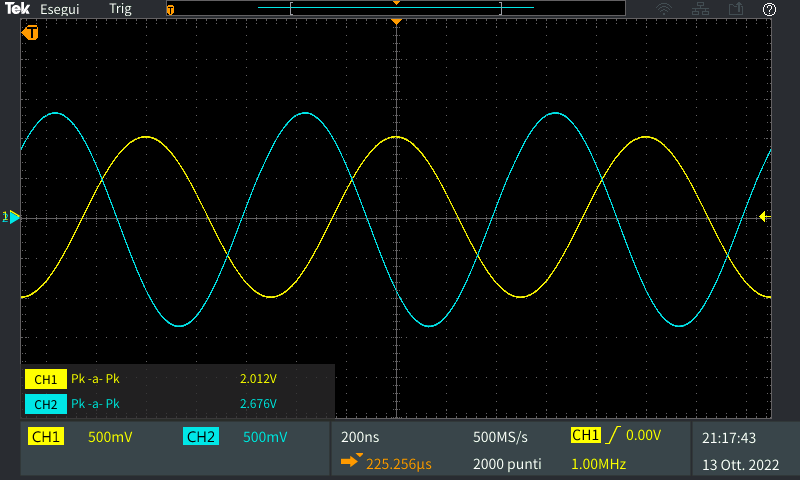
\includegraphics[width=1\linewidth]{./ImageFiles/Laboratorio 2/TEK00050}
	\caption{Misure del segnale $v_{in}$ (linea gialla) e del segnale $v_{1}$ (linea azzurra). Si è utilizzata in ingresso un segnale sinusoidale di ampiezza picco-picco \SI{2}{\volt} con frequenza pari a \SI{1}{\mega\hertz}.}
	\label{fig:analisi_circuito_3_3}
\end{figure}